\renewcommand{\mapa}{Poglavja/Slike/grayscale1000}

\begin{figure}[!ht]
    \centering
    \begin{subfigure}{0.49\linewidth}
        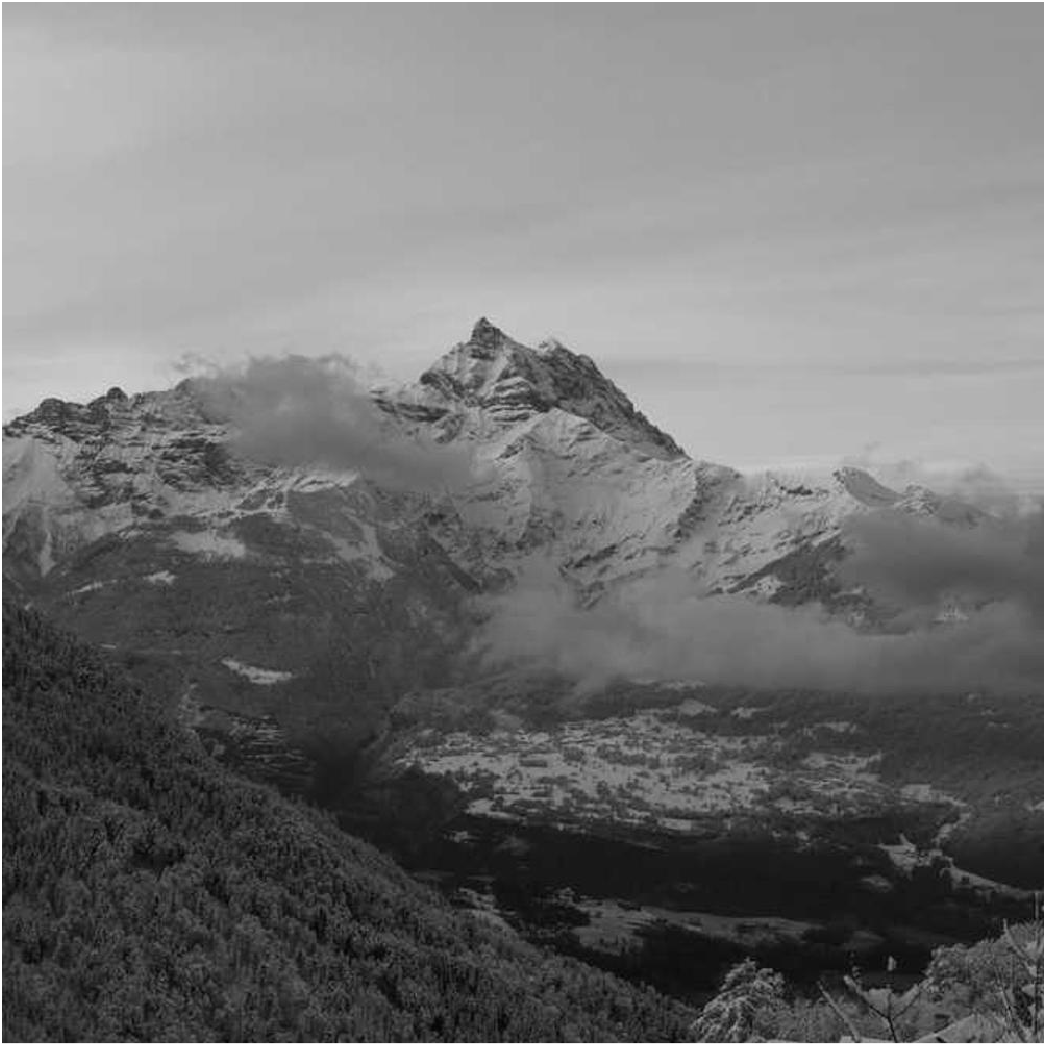
\includegraphics[width=\linewidth]{\mapa/slikaInput.png}
        \caption{Originalna slika}
    \end{subfigure}
    \hfill
    \begin{subfigure}{0.49\linewidth}
        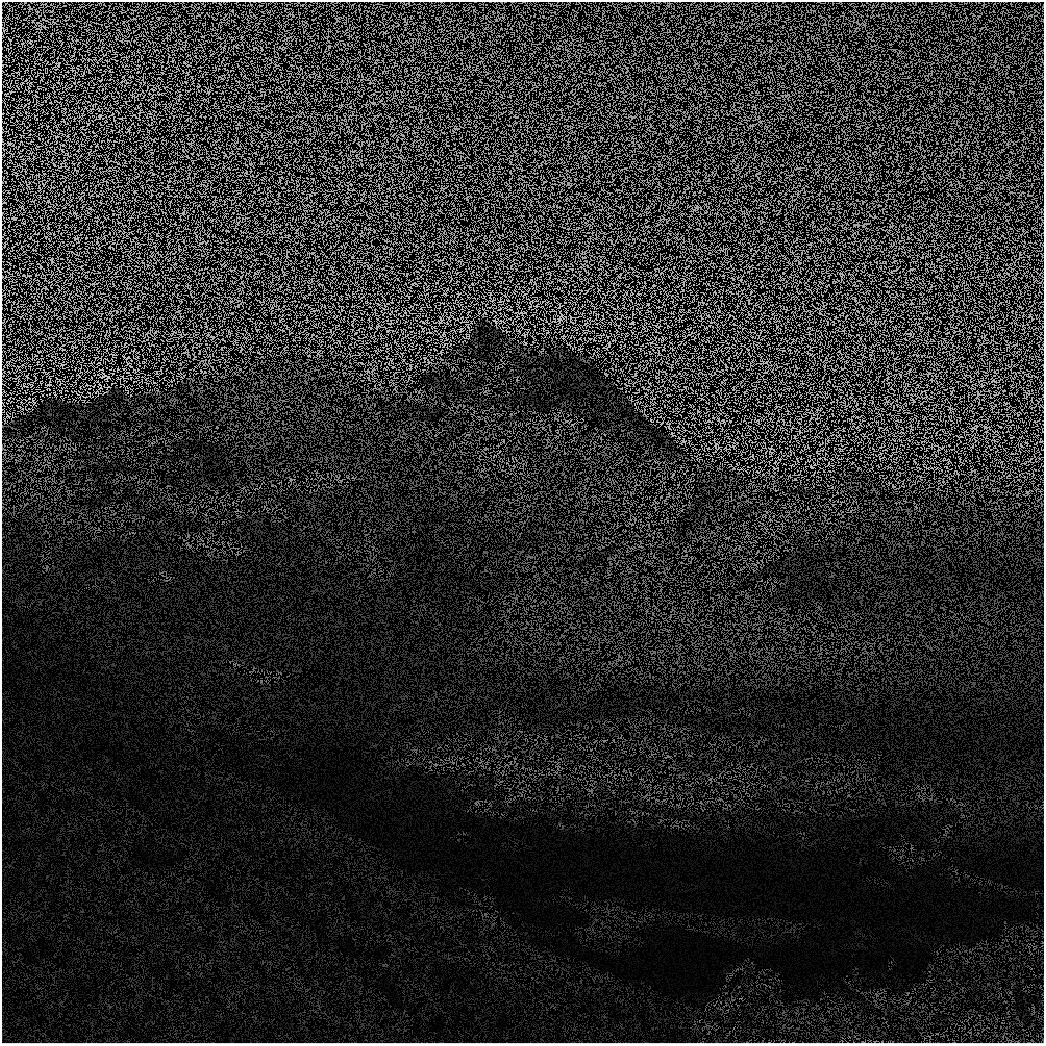
\includegraphics[width=\linewidth]{\mapa/slikaInput35.png}
        \caption{Slika z $0.35$ znanimi podatki}
    \end{subfigure}
    \begin{subfigure}{0.49\linewidth}
        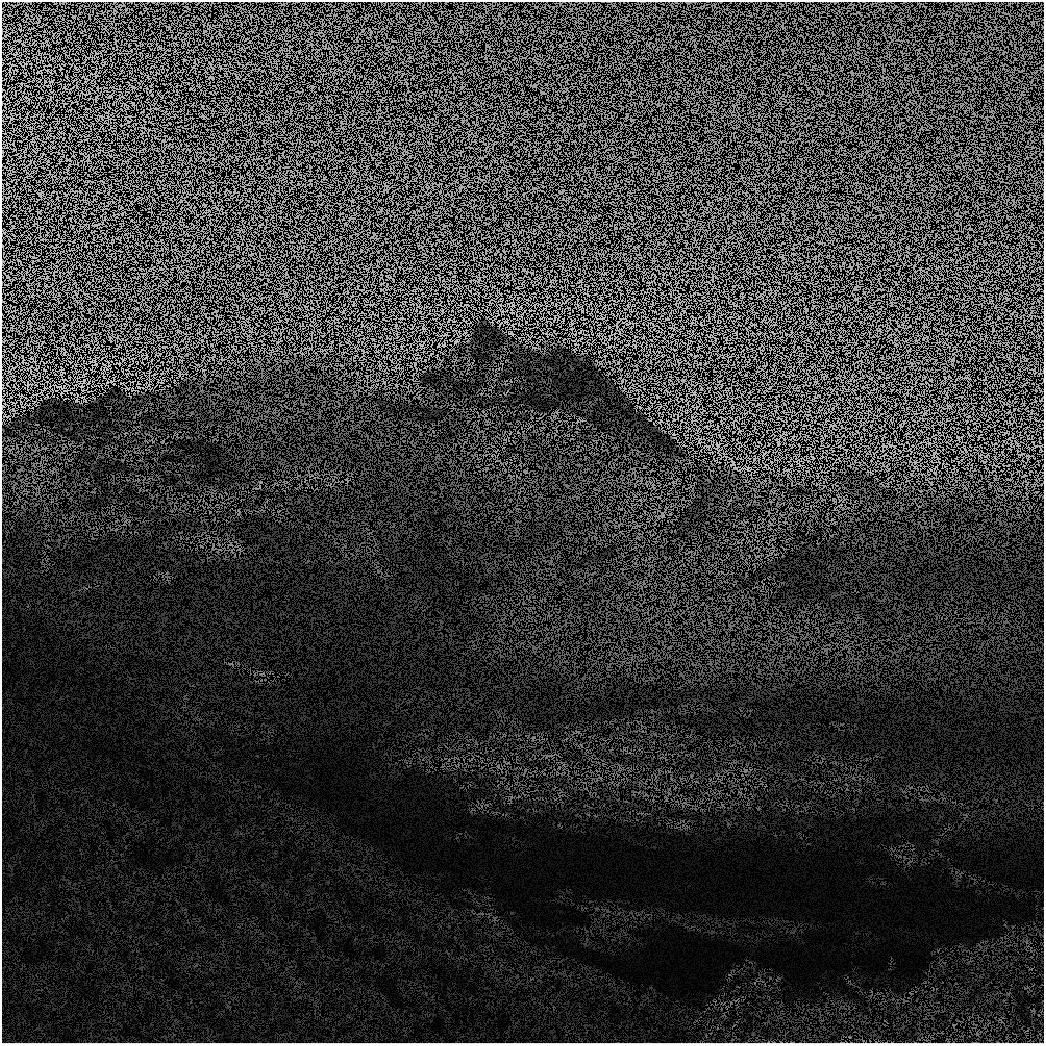
\includegraphics[width=\linewidth]{\mapa/slikaInput45.png}
        \caption{Slika z $0.45$ znanimi podatki}
    \end{subfigure}
    \hfill
    \begin{subfigure}{0.49\linewidth}
        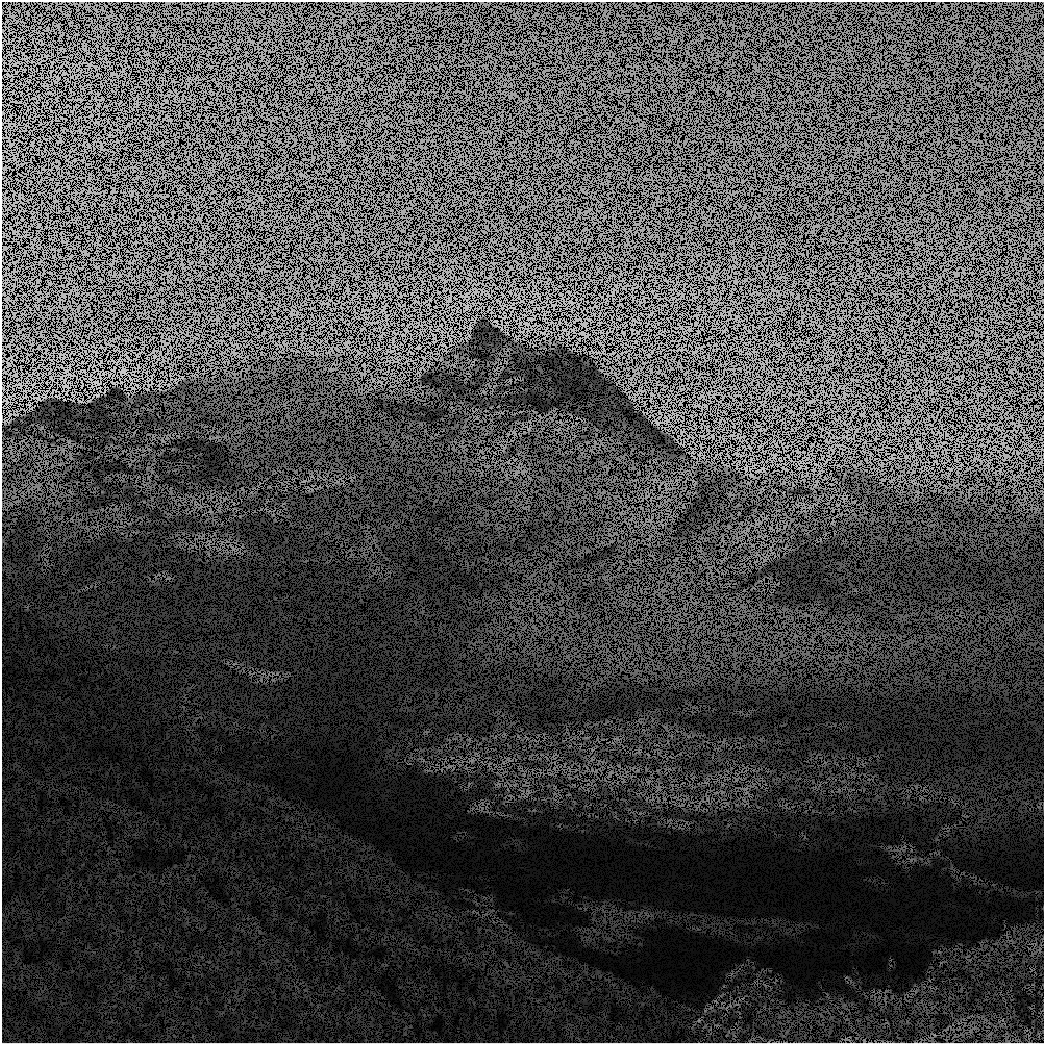
\includegraphics[width=\linewidth]{\mapa/slikaInput60.png}
        \caption{Slika z $0.60$ znanimi podatki}
    \end{subfigure}
    \caption{Vir slike: Unsplash}
\end{figure}

\begin{figure}[!ht]
    \centering
    \begin{subfigure}{0.325\linewidth}
        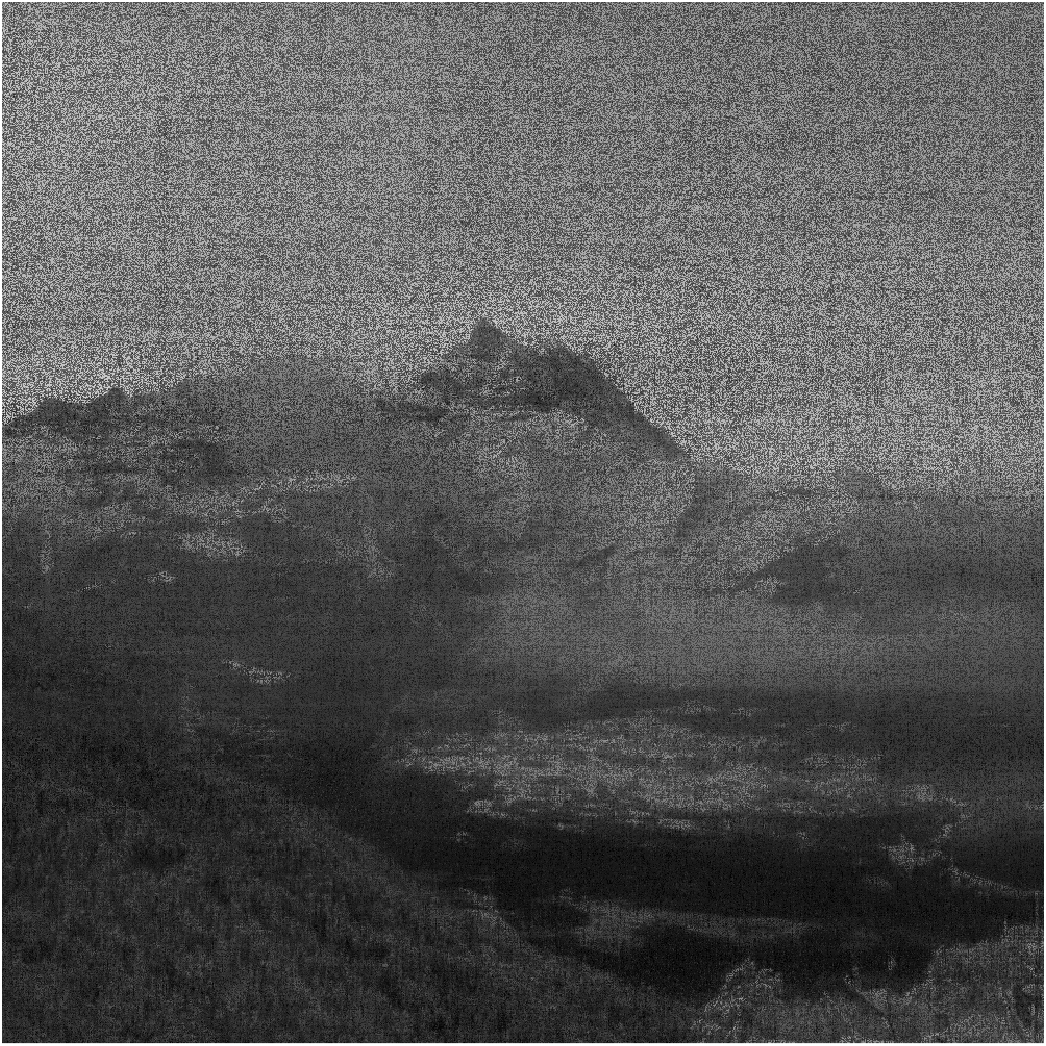
\includegraphics[width=\linewidth]{\mapa/slikaRez35SVT.png}
        \caption{SVT $0.35$}
    \end{subfigure}
    \hfill
    \begin{subfigure}{0.325\linewidth}
        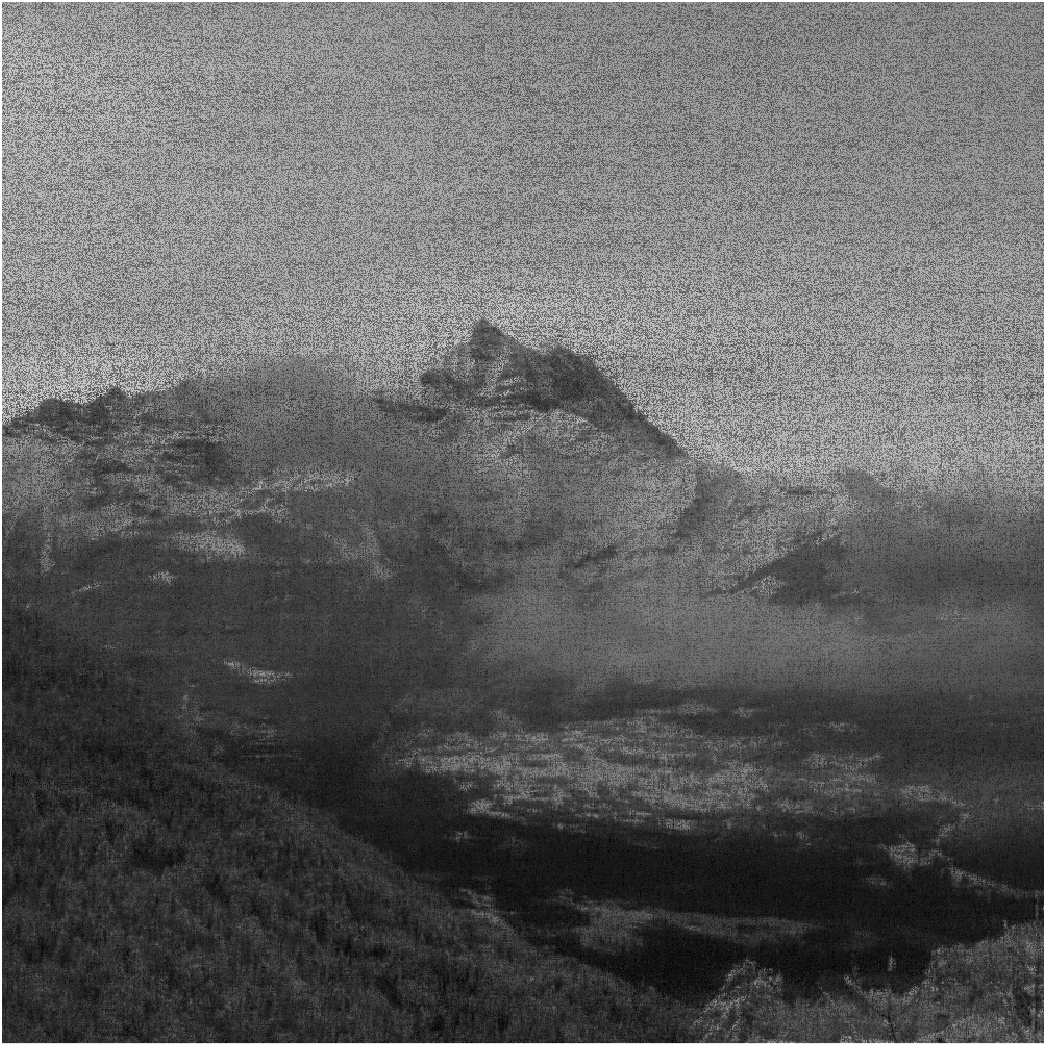
\includegraphics[width=\linewidth]{\mapa/slikaRez45SVT.png}
        \caption{SVT $0.45$}
    \end{subfigure}
    \hfill
    \begin{subfigure}{0.325\linewidth}
        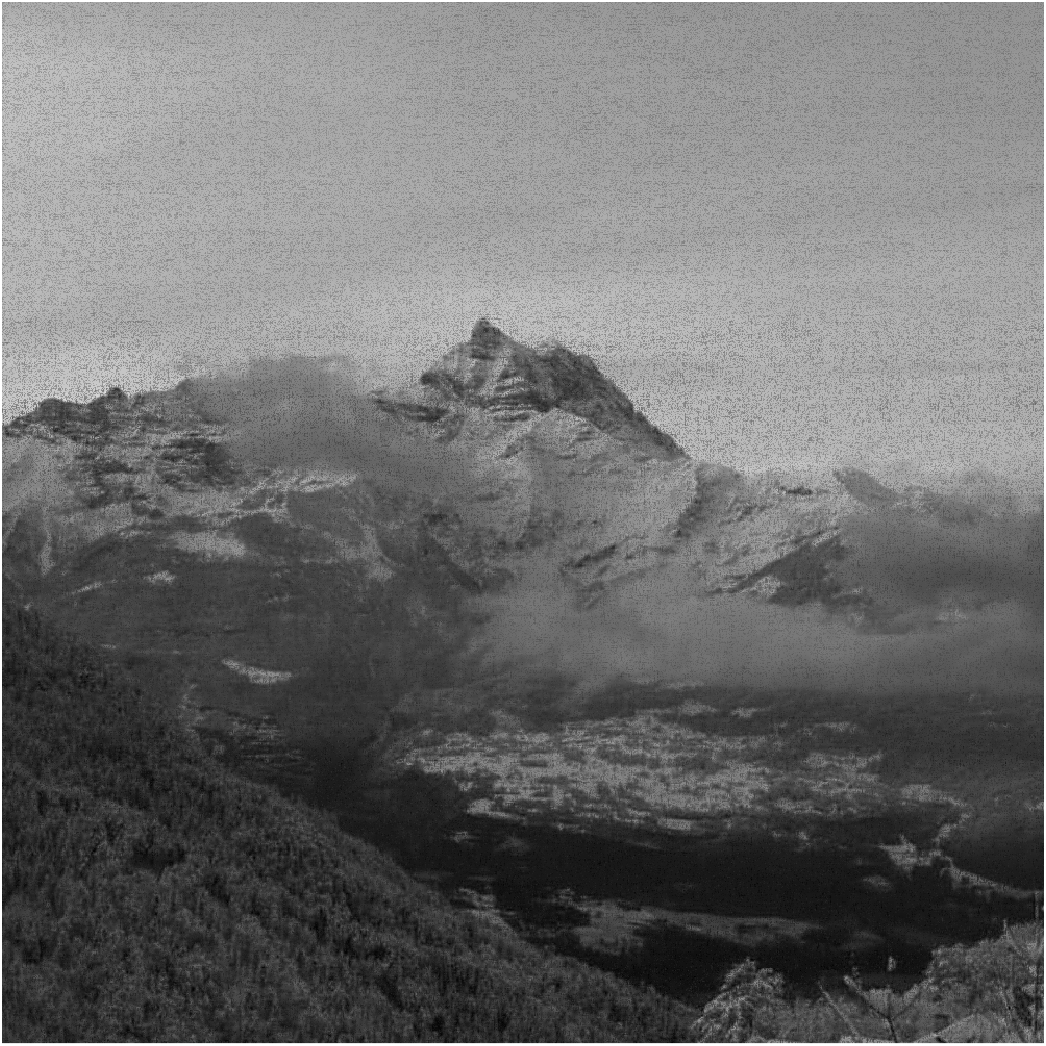
\includegraphics[width=\linewidth]{\mapa/slikaRez60SVT.png}
        \caption{SVT $0.6$}
    \end{subfigure}
    \begin{subfigure}{0.325\linewidth}
        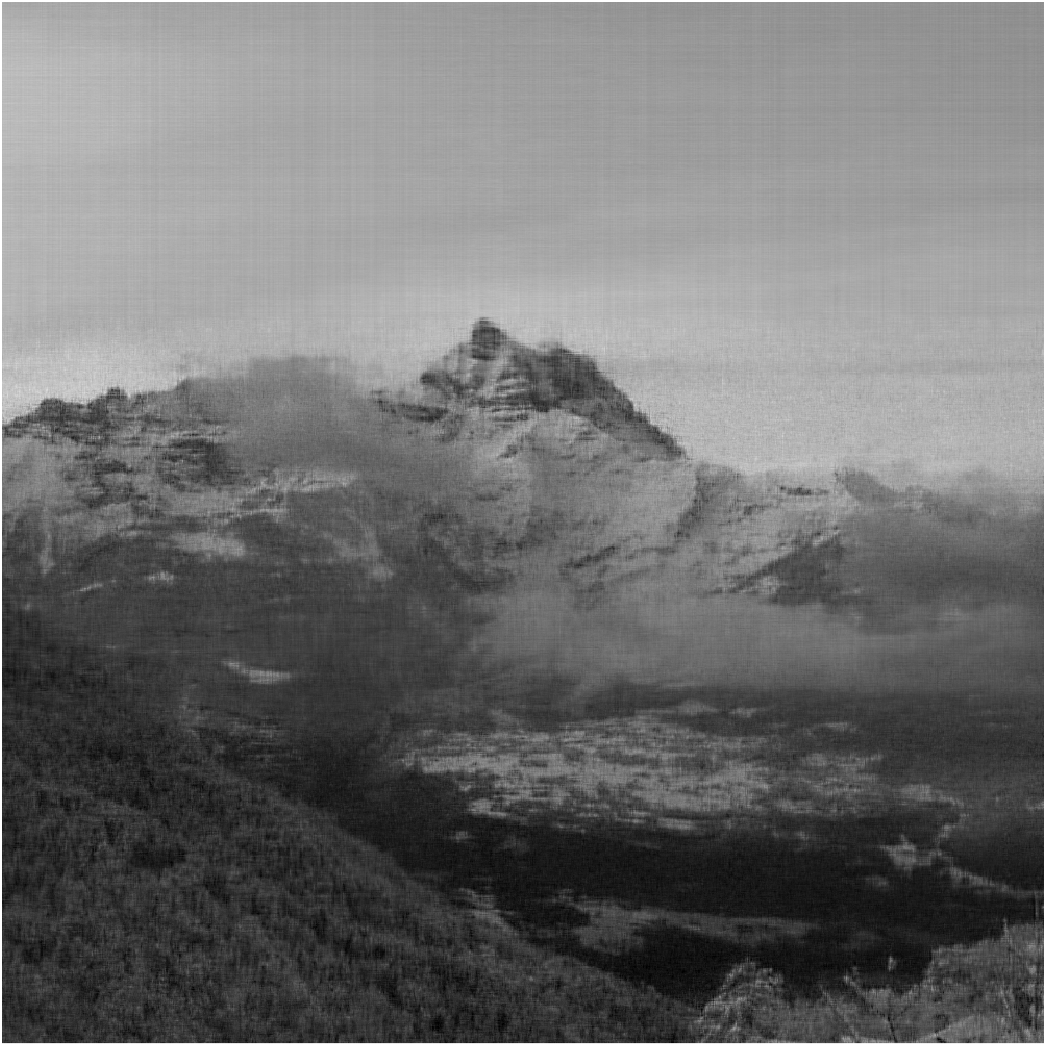
\includegraphics[width=\linewidth]{\mapa/slikaRez35TNNM.png}
        \caption{TNNM $0.35$}
    \end{subfigure}
    \hfill
    \begin{subfigure}{0.325\linewidth}
        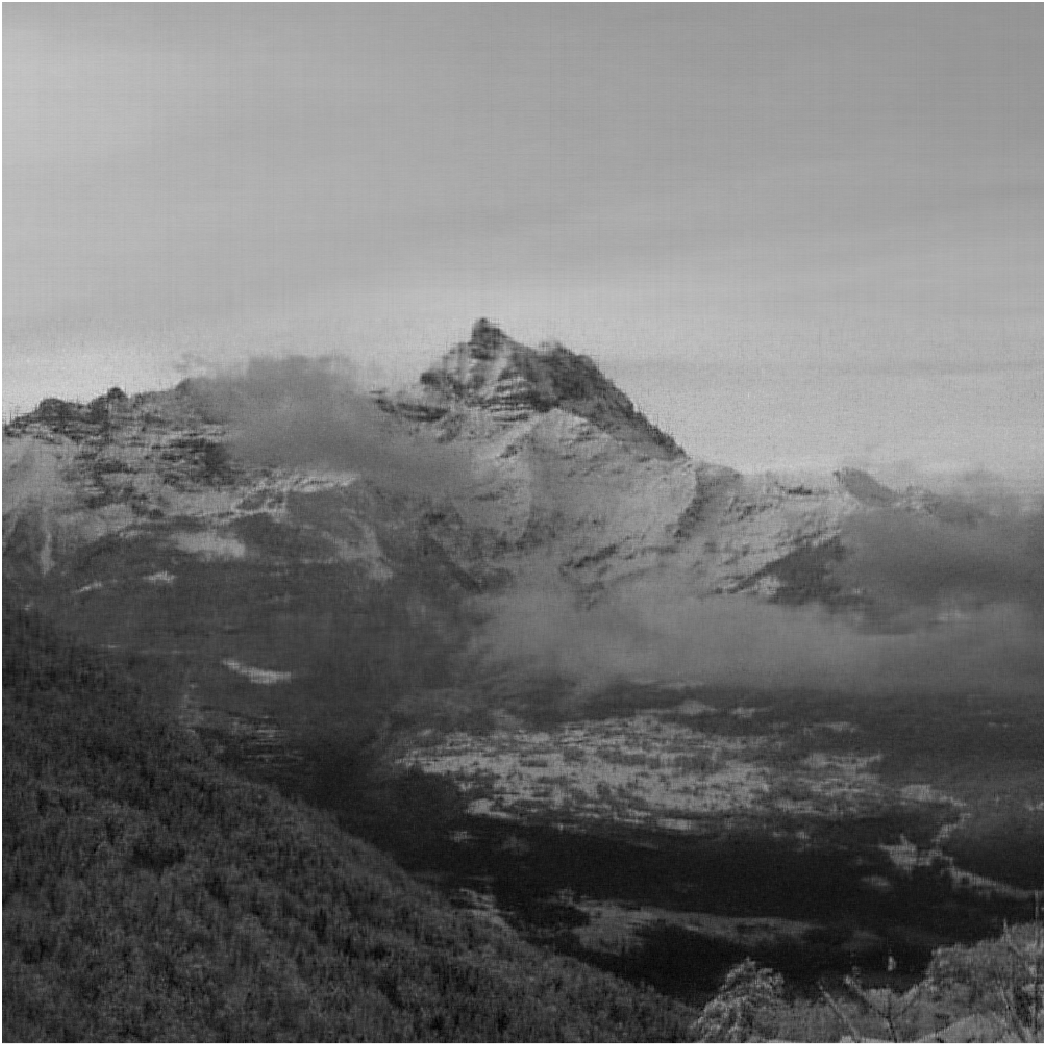
\includegraphics[width=\linewidth]{\mapa/slikaRez45TNNM.png}
        \caption{TNNM $0.45$}
    \end{subfigure}
    \hfill
    \begin{subfigure}{0.325\linewidth}
        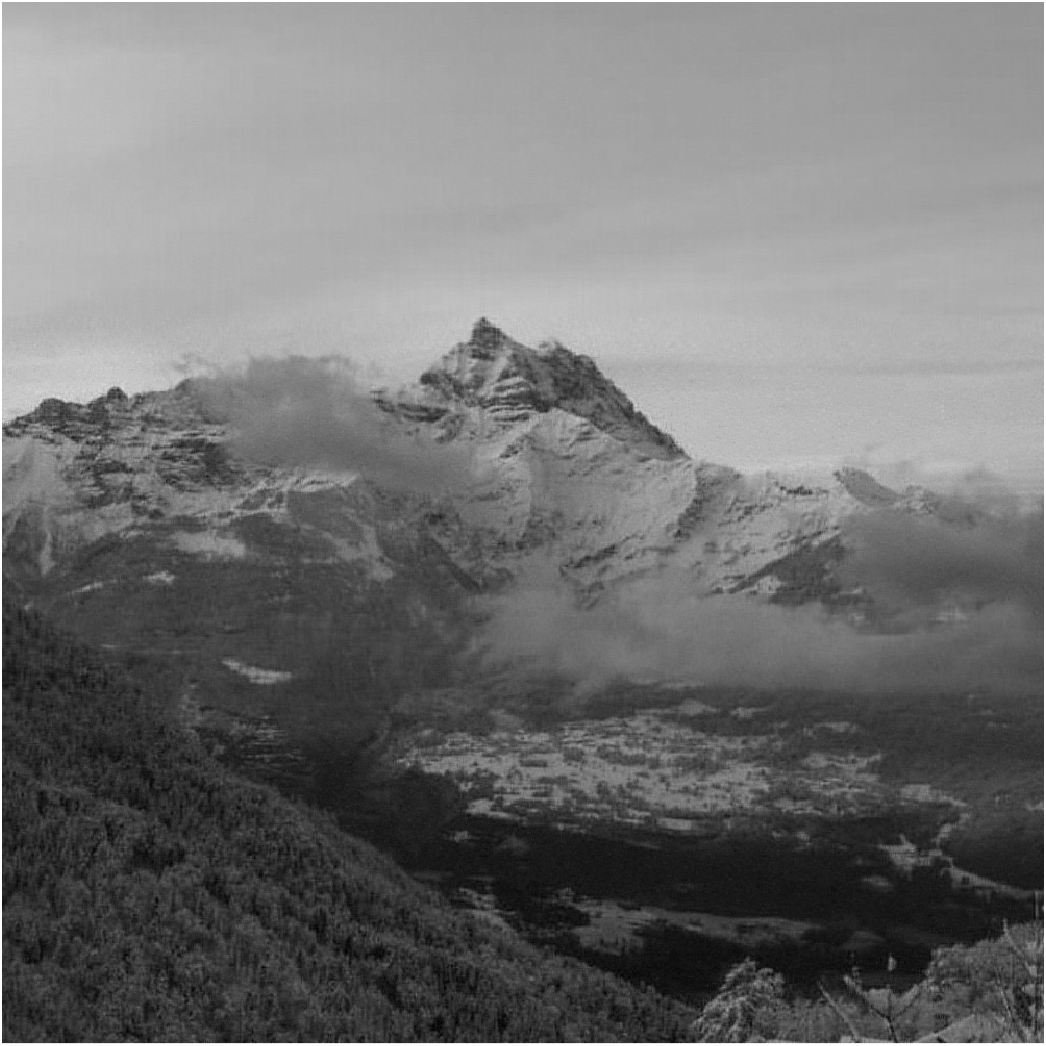
\includegraphics[width=\linewidth]{\mapa/slikaRez60TNNM.png}
        \caption{TNNM $0.6$}
    \end{subfigure}
    \begin{subfigure}{0.325\linewidth}
        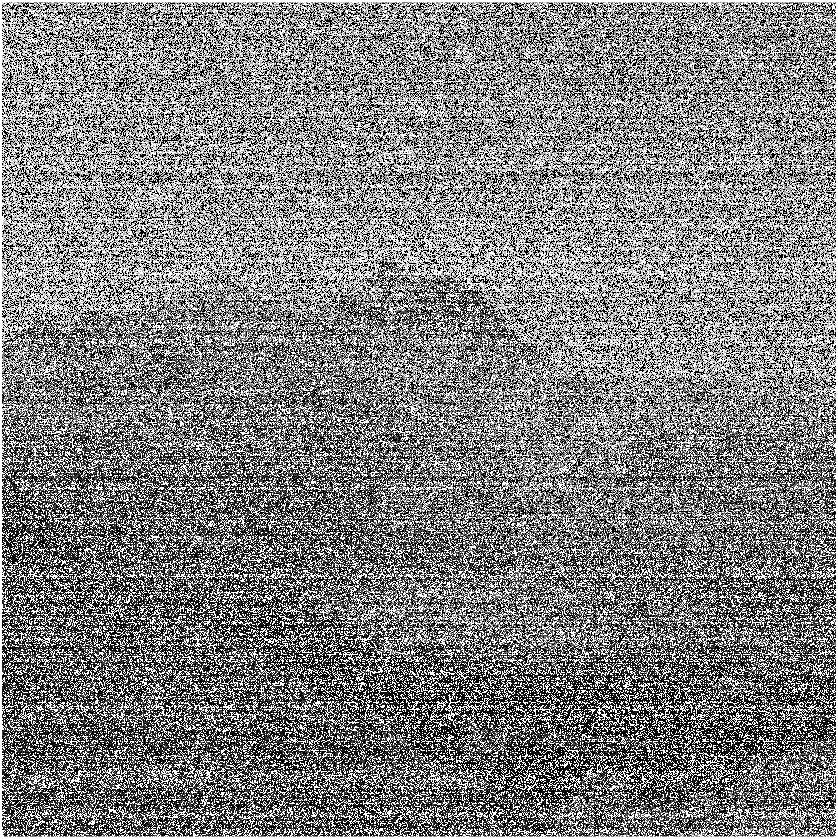
\includegraphics[width=\linewidth]{\mapa/slikaRez35ASD400.png}
        \caption{ASD $0.35$}
    \end{subfigure}
    \hfill
    \begin{subfigure}{0.325\linewidth}
        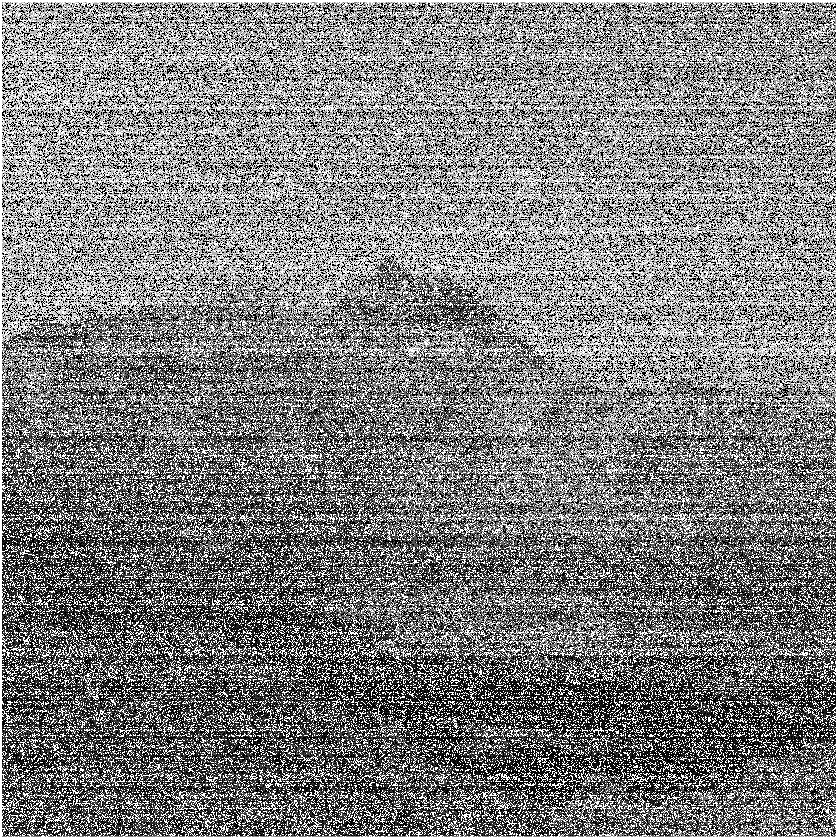
\includegraphics[width=\linewidth]{\mapa/slikaRez45ASD600.png}
        \caption{ASD $0.45$}
    \end{subfigure}
    \begin{subfigure}{0.325\linewidth}
        %ASD 60?%
        \hfill
    \end{subfigure}
    \begin{subfigure}{0.325\linewidth}
        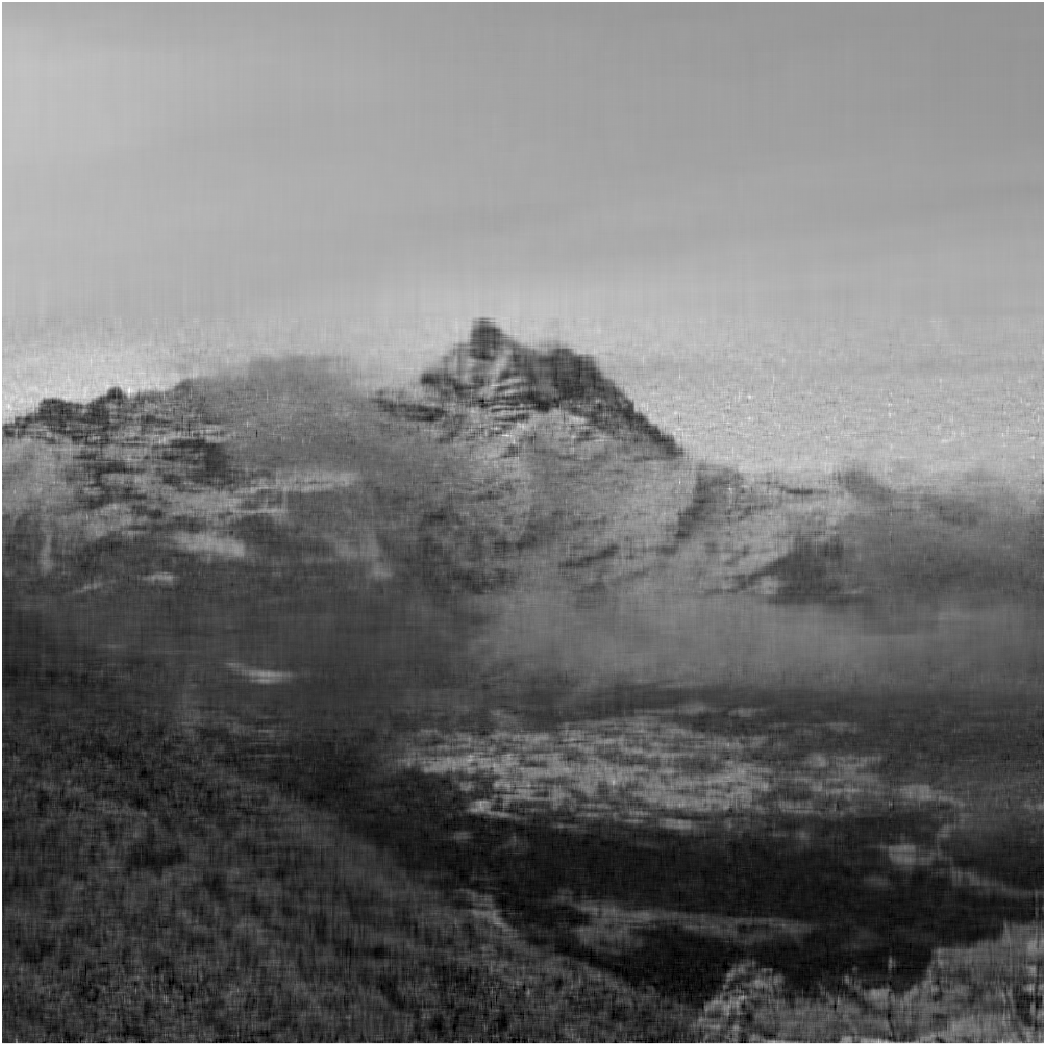
\includegraphics[width=\linewidth]{\mapa/slikaRez35LmaFIT50.png}
        \caption{LMaFit $0.35$}
    \end{subfigure}
    \hfill
    \begin{subfigure}{0.325\linewidth}
        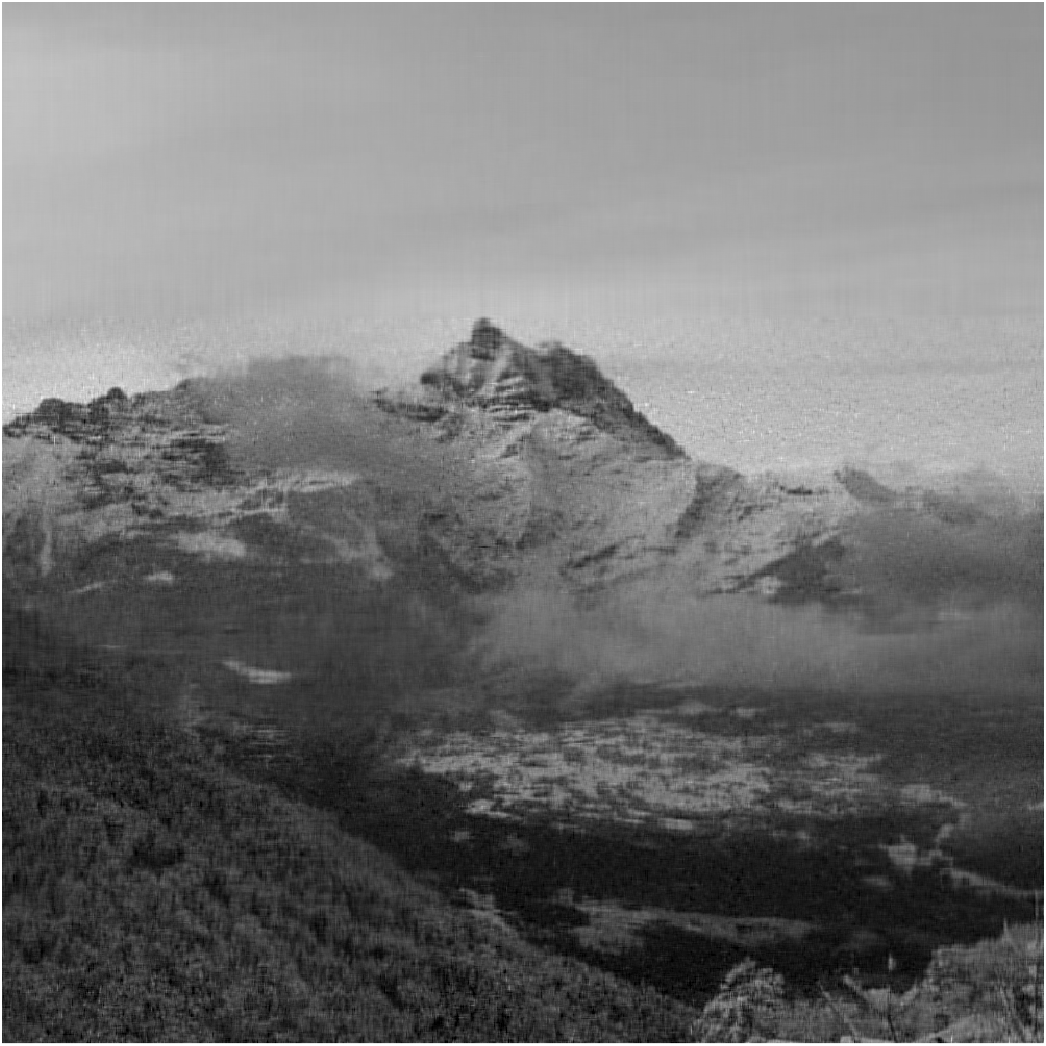
\includegraphics[width=\linewidth]{\mapa/slikaRez45LmaFIT73.png}
        \caption{LMaFit $0.45$}
    \end{subfigure}
    \begin{subfigure}{0.325\linewidth}
        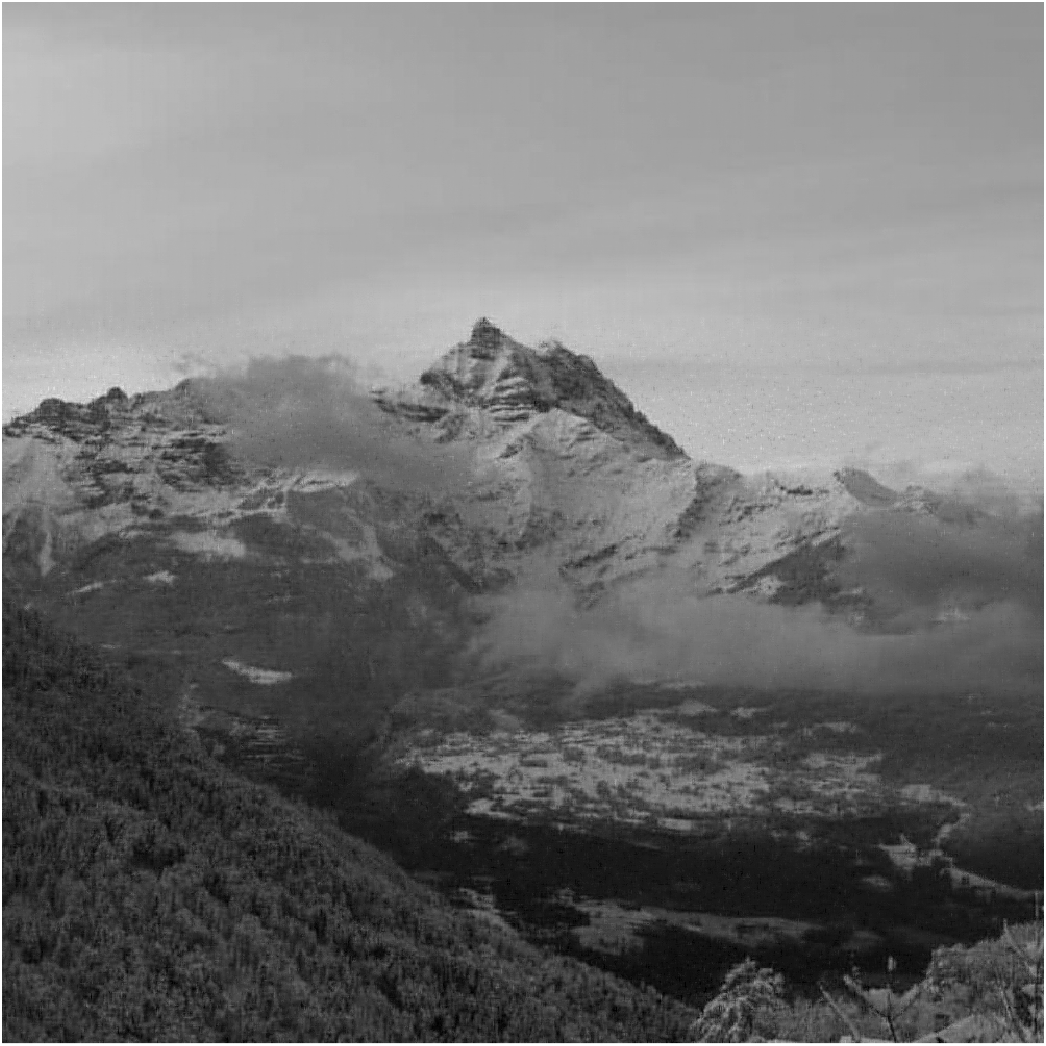
\includegraphics[width=\linewidth]{\mapa/slikaRez60LmaFIT77.png}
        \caption{LMaFit $0.60$}
    \end{subfigure}
\end{figure}